\answer{Explain briefly why the lack of homogeneity is a challenge when
developing distributed systems.}{2}{2014.1.a}

Since most of the individual computers that make up distributed systems will
differ, we need to come up with ways for them to communicate in such a way that
they can have meaningful interactions. This involves creating Interface
Definition Languages, middleware etc to help them inter-operate even when they
might be running different architectures.

\answer{Explain briefly why the assumption “latency is zero” is considered a
common fallacy in distributed computing.}{2}{2014.1.b}

Many (new) programmers haven't created applications intended to use distributed
systems before, and thus don't realise that waiting for a remote resource, RPC
call etc can (will) take orders of magnitude more time than a load from memory
might since it must travel through (many) different systems over different
protocols and even through different countries, where at any stage it may be
delayed and thus the latency increased.

\answer{Explain briefly what publish-subscribe messaging is.}{2}{2014.1.c}

Public-Subscribe messaging is when a `pub-sub' server is designated to take
messages from publishers and forward them to subscribers. The server provides a
central point at which systems can push their messages to and receive their
messages from and know that the message will be sent to/from the correct places.

This is especially handy if one client wishes to push a message to many (or
unknown amounts of) other clients. Instead of having to send $n$ messages, it
can send one message to the pub-sub server and the server will send out the
correct amount of messages to the subscribed clients. This helps abstract the
network topology away from clients.

\answer{In a distributed system, what is the purpose of an IDL?}{2}{2014.1.d}

An Interface Description Language defines an interface with which different
systems who may be running different architectures and different operating
systems etc can serialise data to and from and communicate safely.

They are commonly used by RPC software to facilitate the actual message sending
of the RPC calls.

\answer{In the context of RPC, what is copy-restore and what is it used
for?}{2}{2012.1.e}

Since a local client and a remote server (almost certainly) do not share memory
space, copy-restore is a way of letting one mutate the memory of another
remotely. On making an RPC call, the parameters for the method are serialised
and sent to the receiver, where they are deserialised again. While the procedure
is running, the parameters may be changed, and when the RPC call has finished,
they are serialised and sent back to the original machine, where their new
values are written back to memory.

\answer{What must a server do to provide at most once semantics to its
clients?}{2}{2014.1.f}

It must provide an acknowledgement to clients when it has received an RPC call
and successfully unmarshalled the parameters. This means that clients can know
not to re-sent the RPC call (since otherwise they wouldn't know that it was
received).

See \url{http://stackoverflow.com/questions/13330067/rpc-semantics-what-exactly-is-the-purpose}
for (what looks like) good description of at most once and at least once
semantics.

\answer{Explain briefly what failures are known as Byzantine
failures.}{2}{2014.1.g}

When a remote system either:

\begin{itemize}
  \item Does not reply to messages
  \item Sends faulty replies to message with miscellaneous data
  \item Sends maliciously crafted messages
\end{itemize}

Then it counts as a Byzantine failure.

\answer{In the context of data replication, explain briefly what eventual
consistency is.}{2}{2014.1.h}

When a protocol guarantees that data will eventually be consistent across
multiple systems, but it does not specify a time duration before the data will
be consistent (where consistency means to have the same data values).

\answer{When using Java RMI, what is the purpose of the
rmiregistry?}{2}{2014.1.i}

As a map between a String name of an object and the object's value. Clients can
query the rmiregistry with the name of an object and get the object back. In
this way, it acts as a distributed memory space for distributed systems, since
all systems can read and update the values stored in it.

The rmiregistry means that you aren't limited to just passing values in RPC
calls, you can pass references to objects and datastructures in the rmiregistry
and the system you're calling with the RPC call can look them up in the
rmiregistry.

\answer{In the context of lab exercise 2, what would you do to launch a denial
of service attack against the server?}{2}{2014.1.j}

Find the most expensive operation I can on the server (maybe listing the free
slots), and set up a program on a machine with a fast processor and high
bandwidth to run in a loop sending a request to the server every time it loops.
Thousands or tens of thousands of requests per second could be sent in the right
conditions, which could overload the server, cause it to cease responding (or at
least increase its response times) and deny its service to other users.

\answer{Explain briefly what the role of a client stub and a server stub is in
RPC.}{2}{2014.2.a}

Client stub:

\begin{enumerate}
  \item The client stub receives a request from the client application to
    execute an RPC call.
  \item It marshalls the parameters of the call into a binary or text blob and
    sends it (often in a format specified by an IDL) to the server.
  \item The client waits for a reply.
  \item When a reply is received, the client unmarshalls the parameters and
    updates them in the main memory.
\end{enumerate}

Server stub:

\begin{enumerate}
  \item When the server receives an RPC call from a client, it calls the server
    stub.
  \item The stub unmarshalls the parameters of the call and calls the local
    procedure with them.
  \item Once the procedure is finished, the parameters are marshalled back again
    and sent back to the client.
\end{enumerate}

\answer{Explain briefly what is meant by logical (Lamport) clocks and vector
clocks. What property is captured by vector clocks that is not if Lamport clocks
are used?}{3}{2014.2.b}

Logical and vector clocks aim to provide a happens-before ordering of events in
distributed systems. A logical clock is incremented every time an event occurs
in a distributed system, and it attached to all messages. If a client receives a
message with a higher logical clock than it, then its clock is updated to be
that value, and then it is incremented to signify that an event occurred (a
message received event).

A vector clock is like a logical clock, except each system keeps track of the
clock of each other system in a vector. In this manner, causality is captured by
vector clocks and not by logical clocks.

\answer{Explain briefly what the four properties commonly denoted by the acronym
ACID are when referring to transactions.}{4}{2014.2.c}

\begin{description}
  \item \textit{Atomicity} - Each operation/transaction must either succeed or 
  fail; there is no in-between. If the operation fails, then the state of the
  system must be exactly as it was before the start of the operation.
  \item \textit{Consistency} - Each operation or transaction must bring the
  state of the system from one valid state to another.
  \item \textit{Isolation} - Operations or transactions happening in parallel
  must execute as though they were running in a serial manner.
  \item \textit{Durability} - Once a transaction is committed or an operation
  is completed, the system will not roll back to a previous state in the event
  of failure or power loss etc.
\end{description}

\answer{Describe in detail how a centralised coordinating process can provide a
mutual exclusive access service in a distributed system.}{3}{2014.2.d.i}

A coordinating process acts as a lock server. If a process wants to enter a
section designated to be executed only in a mutually exclusive manner, then it
must first obtain a lock. It does this by asking the lock server for a lock,
executing the mutually exclusive section when it gets it, and releasing the lock
again once its done. If there is already a process in the mutually exclusive
section when another process asks for a lock, the lock server will put the
latter process in a queue until the first has finished with the lock.

\answer{When the machine supporting such a process gets overloaded with
other tasks it needs to find the least loaded machine in the network, and
pass over the provision of the mutual exclusive access service to a
process on that machine. Two algorithms are being considered for this.
The first is to have the server ask each machine about its workload and
then notify all the clients with the identity of the new server. The
second is to use a ring-based election, initiated by the current
server.}{8}{2012.2.d.ii}

\textbf{Fully describe the latter, clearly stating any assumptions you make and
compare it with the former with respect to the number of messages passed.}

A ring based election proceeds as follows:

\begin{enumerate}
  \item The initiator of the election will send a message to the next node
    containing its identifier (a pair of the name of the server and the
    reciprocal of its load).
  \item Each node will then forward the message if its identifier (the load) is
    lower than that of the message, or send its own identifier if its higher.
  \item The message goes around the circle until one node receives its own
    identifier.
  \item This means that the message has gone once around the ring and no other
    machine is more eligible for the role of coordinator, so the receiving
    machine considers itself elected.
  \item The newly elected coordinator then sends a message around the ring 
    announcing its election.
\end{enumerate}

The assumptions are that messages are sent reliably, and that no processes
crash.

This takes $O(3n-1)$ messages in the worst case, whereas the more simpler one
takes $O(3(n-1)) = O(3n - 3)$ messages, which although two fewer messages are
sent, is potentially worse since it requires each server to know about all other
servers.

\answer{Describe clearly all the operations that take place during a Remote
Procedure Call (RPC).}{4}{2014.3.a}

First, the client application will call the client stub with the procedure it
wants to execute and the parameters that are needed to do so. The client stub
then marshalls the parameters into a blob which is then sent to the server. The
server receives the message and the server stub unmarshalls the blob back into
parameters, which are then passed to the procedure on the server and the
procedure is ran. When the procedure is finished the server stub marshalls the
(possibly mutated) parameters back into a blob and sends it back to the client,
where the client stub will then unmarshal the parameters, update their values
in main memory and return to the client application.

\answer{Two computers are used to provide a replicated service. Each computer
has a mean time between failures of 12 days; a failure takes on average 12 hours
to fix. What is the availability of the replicated service?}{3}{2014.3.b}

Probability of failure = $1 - \frac{12}{(12 * 24) + 12} = 0.96$.

The probability of both machines failing at the same time is $0.96^2 = 0.9216 =
92.16\%$.

\answer{Consider a client-server application, which consists of 100 services
provided by some server. Ten of these services must be executed strictly one
after the other, not in parallel with any other services. The remaining 90
services may be executed concurrently and in any order. Assume that each service
takes the same time to execute. What is the maximum speedup that can be obtained
for the application if multiple identical servers are used to provide the
required services?}{3}{2014.3.c}

If ten services have to be executed in a serial manner, and the last 90 can be
executed in parallel then the maximum speed up using a number of parallel
processors is (using Amdahl's law):

\[
  \text{speedup} = \frac{1}{0.1 + (\frac{1}{\infty} * 0.9)} = 10\times
\]

\answer{Consider a simple server that carries out client requests without
accessing other servers. Explain why it is generally not possible to set a limit
on the time taken by such a server to respond to a client request. What would
need to be done to make the server able to execute requests within a bounded
time?}{4}{2014.3.d}

Since latency is variable, although we could try and ensure that the server
sends a response back to the client $n$ seconds after it has received a request,
we cannot make guarantees about how long it will take for the message to get
from the client to the server and back again.

Furthermore, we don't know how many requests the server might be dealing with, if
it has a queue of 1000000 requests, then it probably won't reply in the bounded
time.

The only way we might make such guarantees is by taking control of the network
and implementing some path through which packets can get from the client to the
server within a bounded time, and scaling the service horizontally so that more
server processes are online if the queue of requests starts to get large.

\answer{The following two processes access the shared variables x, y, z. Each
process accesses a different replica of the store used to hold these variables.
Before any process starts executing, the value of all three variables, x, y, z,
is 0 in all the replicas.}{6}{2014.3.e}

\begin{center}
  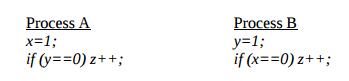
\includegraphics[width=0.4\textwidth]{images/2014-3-d}
\end{center}

\answer{When both processes have completed executing the statements given,
what are the possible values of z, if the replication uses the sequential
consistency model? Justify your answer.}{3}{2014.3.d.i}

If process A executes first, then the value of $z$ will be 1, and if process B
executes first then the value of $z$ will still be 1. This is because in both
cases, the \texttt{if} statement on the second process will fail.

\answer{When both processes have completed executing the statements given,
what are the possible values of z, if the replication uses the causal
consistency model? Justify your answer.}{3}{2014.3.d.ii}

The possible values are $z = {0,1}$ since if the statements $x=1;y=1;$ are
executed first, then both if statements will fail and $z=0$, if one process
fully executes before the other starts, then it will be the same case as in
\texttt{d.i}, and $z=1$, but $z$ can never be $2$ because either $x=1$ or $y=1$
before two of the if statements can be reached, so $z$ can never be incremented
twice.
